\section{Проектирование программного средства}
\label{sec:design}

Проектирование – процесс определения архитектуры, компонентов, интерфейсов и других характеристик системы или её части. Результатом проектирования является проект – целостная совокупность моделей, свойств или характеристик, описанных в форме, пригодной для последующей реализации системы. Оно, наряду с анализом требований, является частью большой стадии жизненного цикла системы, называемой определением системы. 

Проектирование системы направлено на представление системы, соответствующее предусмотренной цели, принципам и замыслам; оно включает оценку и принятие решений по выбору таких компонентов системы, которые отвечают её архитектуре и укладываются в предписанные ограничения.

\subsection{Проектирование алгоритма работы программы}
\label{sec:design:algorithm}

На рисунке~\ref{sec:design:main_algorithm_scheme} представлена схема алгоритма работы программного средства создания веб-приложений с помощью готовых графических компонентов. 
На ней отражены такие возможные действия, доступные для выполнения, как рисование, подключение, отправка голосовых данных и отключение. 

В зависимости от конкретного действия, каждое содержит в себе собственные шаги реализации. Так при выборе действия "Применение компонента" происходит отрисовка одного компонента, перетянутого пользователем на грид-разметку, а при выборе "Применение пресета" происходит отрисовка целой совокупности компонентов. "Редактирование свойств" содержит в себе проверку введённых данных на корректность и процесс измненения свойств выбранного компонента. "Удаление компонента" осуществляется при выбора компонента и нажатии кнопки удаления, в таком случае все дочерние элементы (если они есть) также удаляются, после чего родительский компонент (если выбранный удаляемый компонент не был помещен непосредственно на грид-разметку) также перерисовывается. Каждое действие влечет за собой дополнительное действие в виде запоминания выполненных действий в истории изменений, чтобы в случае необходимости "откатить" произошедшие изменения.\pagebreak

\begin{figure}
\centering
    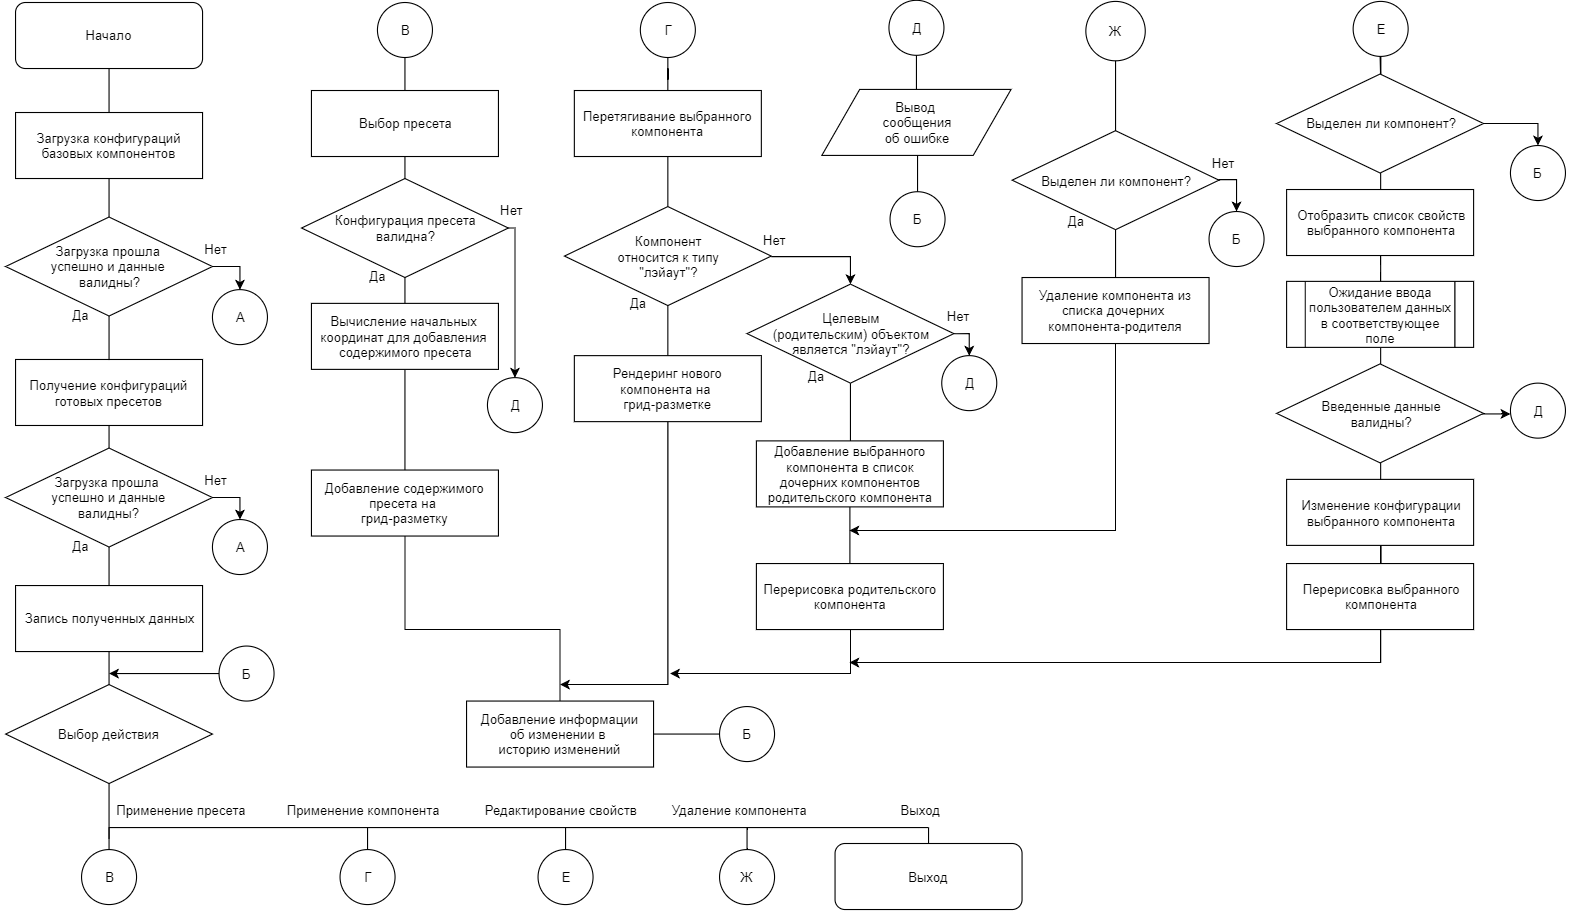
\includegraphics[scale=0.40]{Main_algorithm_scheme.png}
    \caption{Диаграмма прецедентов приложения}
    \label{sec:design:main_algorithm_scheme}
\end{figure}

\subsection{Диаграмма прецедентов приложения}
\label{sec:design:algorithm}

Диаграмма прецедентов в UML диаграмма, отражающая отношения между актёрами и прецедентами и являющаяся составной частью модели прецедентов, позволяющей описать систему на концептуальном уровне.

Прецедент, также: вариант использования, сценарий использования — спецификация последовательностей действий (варианты последовательностей и ошибочные последовательности) в Унифицированном языке моделирования (UML), которые может осуществлять система, подсистема или класс, взаимодействуя с внешними действующими лицами.

Сформируем модель вариантов использования разрабатываемой системы (рисунок~\ref{sec:design:use_case}).

Основным актером, взаимодействующим с системой, является <<Пользователь>>, который взаимодействует с приложением Conference Viewer. Данный пользователь, используя графический интерфейс данного программного средства, получает доступ к его функциям.

Ограничение функциональности для пользователей могут определять разработчики, интегрирующие данный программный модуль свое программное средство. Да и потом, сами разработчики могут в процессе разработки пользоваться данным инструментом с целью ускорения процесса разработки путем автоматизации тривиальных действий создания графический компонентов.\pagebreak

На основании диаграммы прецедентов программного средства, изображенной на рисунке~\ref{sec:design:use_case} можно выделить следующие сценарии его использования:
\begin{itemize}
    \item применение пресета из списка доступных;
    \item очистить грид-разметку;
    \item отменить предыдущее действие;
    \item переключить текущий вид, используя меню;
    \item изменить размер сетки грид-разметки;
    \item применить компонент путем перетаскивания нужного из списка компонентов на грид-разметку;
    \item сохранить пресет;
    \item сгенерировать код приложения;
    \item выбрать компонент и применить в его отношении изменения.
\end{itemize}

\begin{figure}
\centering
    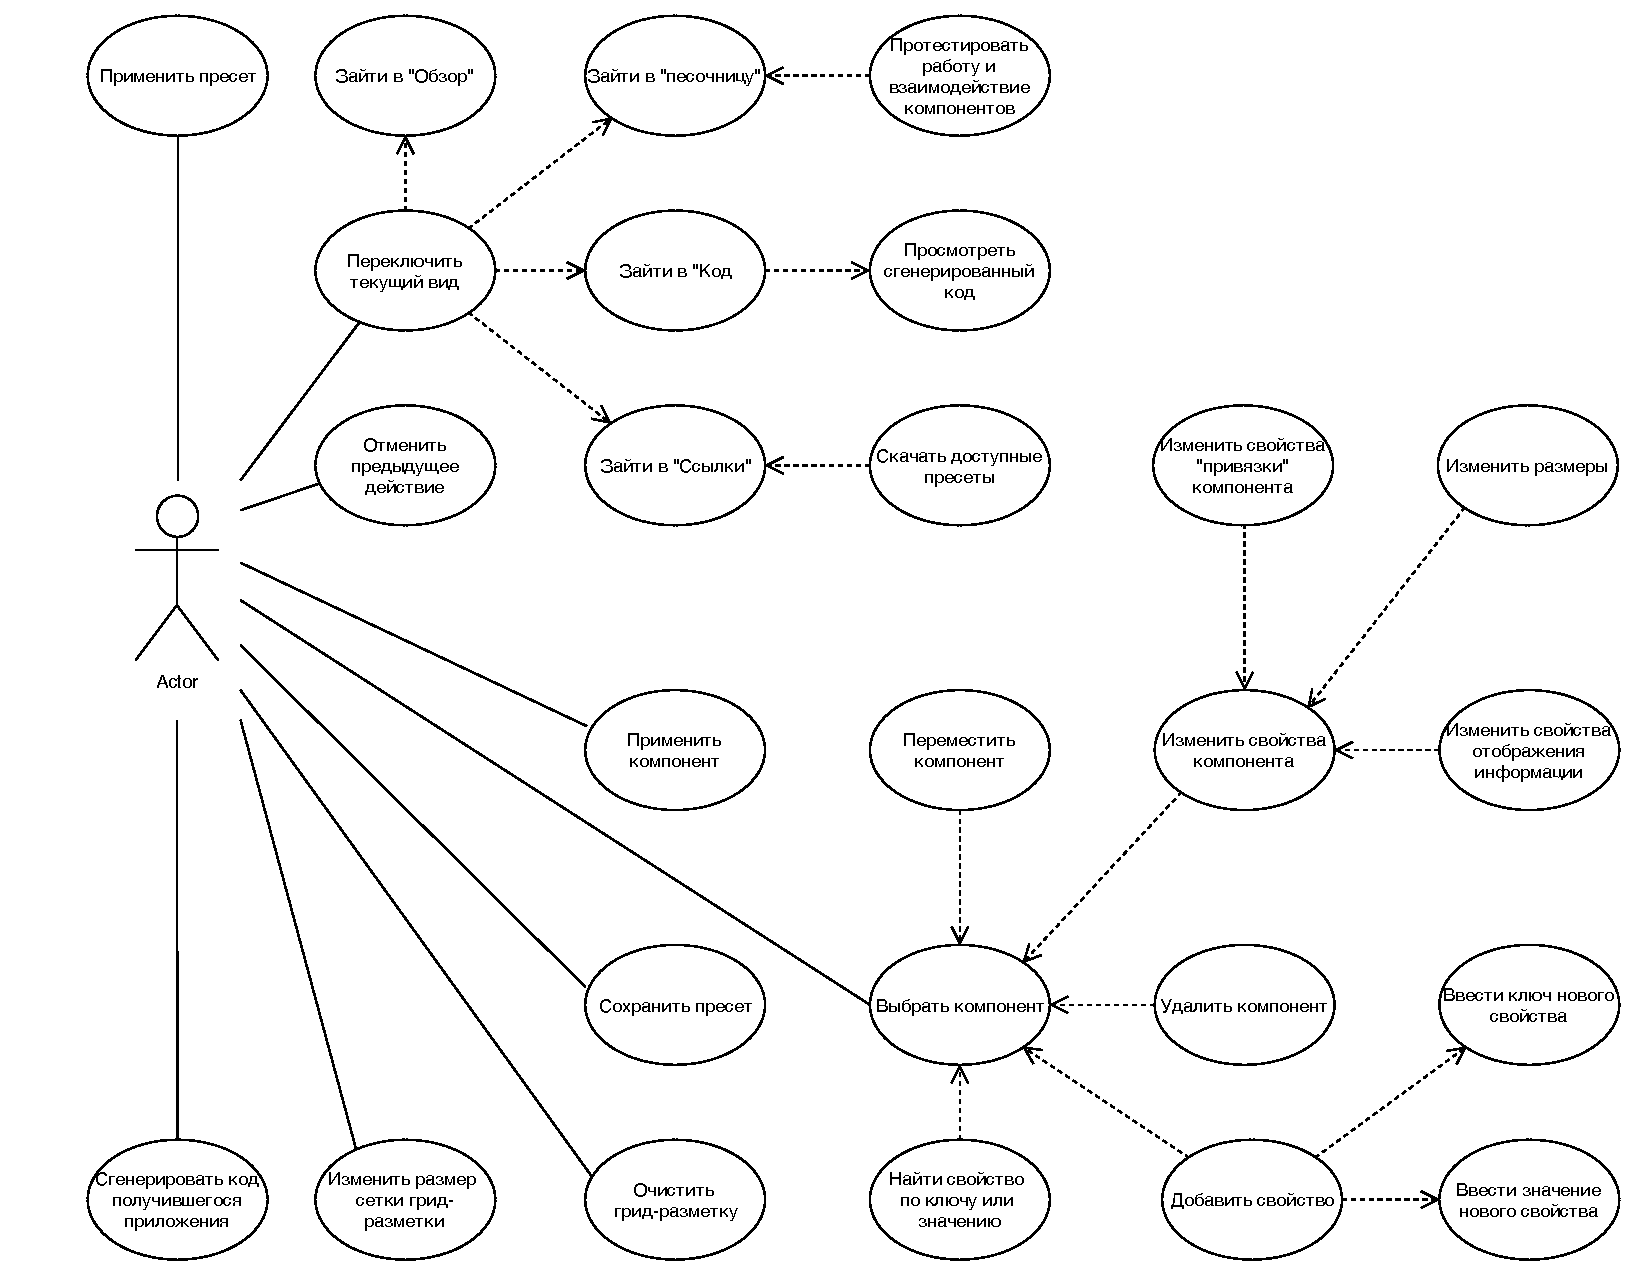
\includegraphics[scale=0.40]{Use_case.pdf}
    \caption{Диаграмма прецедентов приложения}
    \label{sec:design:use_case}
\end{figure}

